%&encoding=UTF-8 Unicode
\documentclass{beamer}

\mode<presentation> {
    \usetheme[compress]{Amsterdam}
    \setbeamercovered{transparent}
}

\usepackage{ucs}
\usepackage[utf8]{inputenc}
\usepackage[czech]{babel}
\usepackage{palatino}
\usepackage{graphicx}
\usepackage{epstopdf}
\usepackage{minted}

\AtBeginSection[]%
{%
\begin{frame}%
  \begin{center}%
    \usebeamerfont{section title}\insertsection%
  \end{center}%
\end{frame}%
}

\usemintedstyle{trac}

\title{E-puck knihovna pro Python}
\author{David Marek}
\institute[MFF UK]{Univerzita Karlova v Praze}
\date{5.~4.~2011}

\begin{document}

\begin{frame}
    \titlepage
\end{frame}

\begin{frame}
    \frametitle{Osnova}
    \tableofcontents
\end{frame}

\section{Představení e-puck robota}

\begin{frame}
    \frametitle{E-Puck}
    \begin{columns}
        \begin{column}{.6\textwidth}
            \begin{itemize}
                \item Ecole Polytechnique Fédérale de Lausanne
                \item Miniaturní robot (průměr 75mm)
                \item Opensource hardware
                \item Spousta senzorů
                \item Bluetooth komunikace
                \item Dostupný (v labu)
            \end{itemize}
        \end{column}

        \begin{column}{.4\textwidth}
            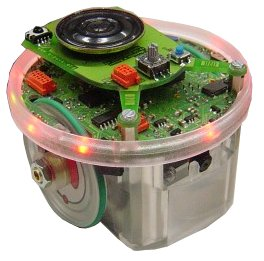
\includegraphics[scale=0.4]{e-puck.jpg}
        \end{column}
    \end{columns}
\end{frame}


\begin{frame}
    \frametitle{Senzory a akční členy}
    \begin{itemize}
        \item Kamera (640x480)
        \item IR senzory (proximity / ambient light)
        \item Akcelerometr (3D)
        \item Mikrofony
        \item LED
        \item Krokové motory
        \item Speaker
    \end{itemize}
\end{frame}

\begin{frame}
    \frametitle{Kamera}
    \begin{columns}
        \begin{column}{.7\textwidth}
            \begin{itemize}
                \item Rozlišení 640x480
                \item Dva režimy: RGB565 / barvy šedi
                \item Příliš velké fotky pro zpracování v robotovi
                \item Řešení problémů s pamětí:
                    \begin{itemize}
                        \item Prokládání
                        \item Změna formátu fotografie
                    \end{itemize}
                \item Reálně jde získat:
                    \begin{itemize}
                        \item 40x40 barevně
                        \item 55x55 černobíle
                        \item Lineární kamera
                    \end{itemize}
            \end{itemize}
        \end{column}

        \begin{column}[c]{.3\textwidth}
            \begin{center}
                \hspace{-2cm}
\includegraphics{fotka1.jpg}\\
                \vspace{0.3cm}
                \hspace{-2cm}
\includegraphics{fotka2.jpg}\\
                \vspace{0.3cm}
                \hspace{-2cm}
\includegraphics{fotka3.jpg}\\
                \vspace{0.3cm}
                \hspace{-2cm}
\includegraphics[scale=0.4]{fotka4.jpg}
            \end{center}
        \end{column}
    \end{columns}
\end{frame}

\begin{frame}
    \frametitle{IR senzory}
    \begin{columns}
        \begin{column}{0.6\textwidth}
            \begin{itemize}
                \item 8 senzorů po obvodu
                \item Dva režimy:
                    \begin{itemize}
                        \item Aktivní -- rozeznávání překážek
                        \item Pasivní -- intenzita světla
                    \end{itemize}
                \item Překážky do $\sim$ 4cm
            \end{itemize}
        \end{column}

        \begin{column}{0.4\textwidth}
            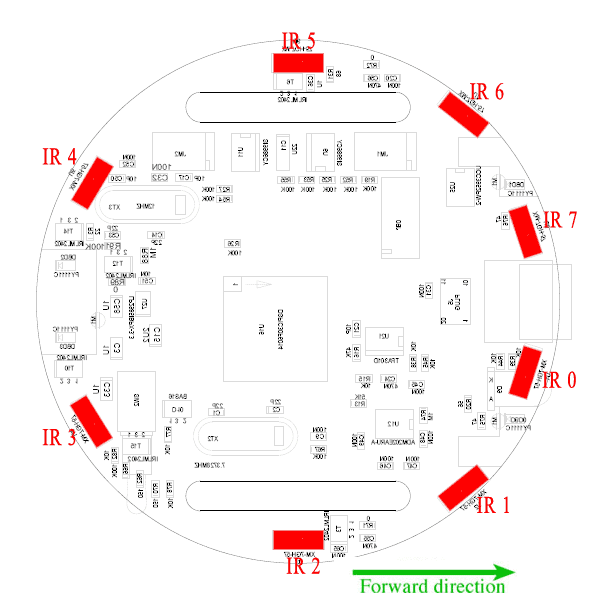
\includegraphics[scale=0.2]{proximity_emplacement.png}
        \end{column}
    \end{columns}
\end{frame}

\begin{frame}
    \frametitle{Akcelerometr}
    \begin{columns}
        \begin{column}{0.6\textwidth}
            \begin{itemize}
                \item 3D akcelerometr
                \item Z robota se dá získat:
                    \begin{itemize}
                        \item Vektor akcelerace
                        \item Zpracované informace (rotace, zrychlení, \ldots)
                    \end{itemize}
                \item Detekce nárazu, naklonění, směru pohybu
            \end{itemize}
        \end{column}

        \begin{column}{0.4\textwidth}
            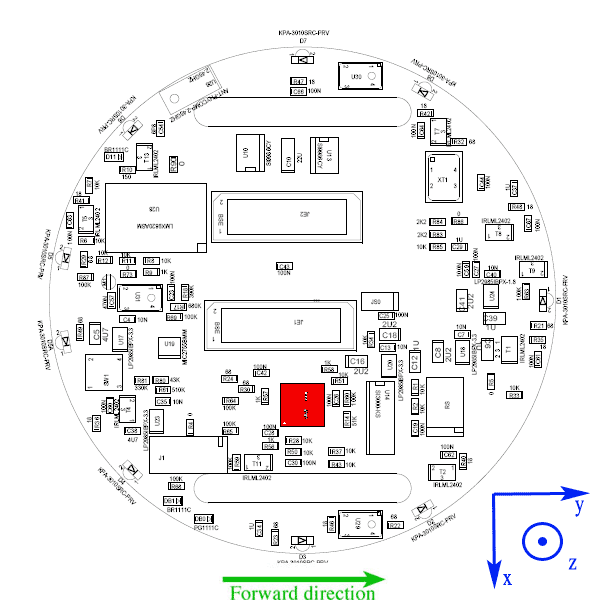
\includegraphics[scale=0.2]{acc_emplacement.png}
        \end{column}
    \end{columns}
\end{frame}

\begin{frame}
    \frametitle{Mikrofony}
    \begin{columns}
        \begin{column}{0.6\textwidth}
            \begin{itemize}
                \item 3 mikrofony
                \item Vlevo, vpravo, vzadu
                \item Lze získat:
                \begin{itemize}
                    \item Hlasitost
                    \item Frekvenci (FFT)
                \end{itemize}
            \end{itemize}
        \end{column}

        \begin{column}{0.4\textwidth}
            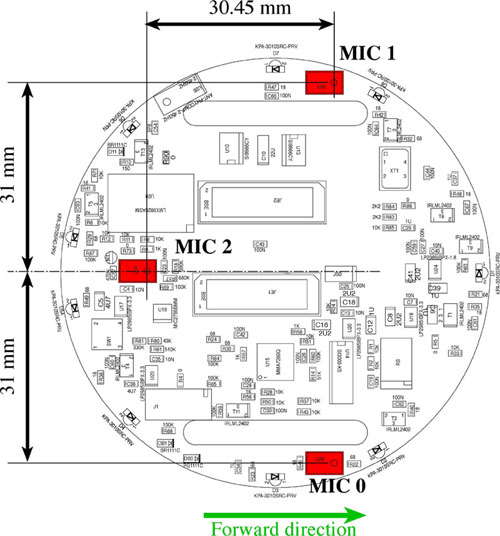
\includegraphics[scale=1]{sound.jpg}
        \end{column}
    \end{columns}
\end{frame}

\begin{frame}
    \frametitle{LED}
    \begin{columns}
        \begin{column}{0.5\textwidth}
            \begin{itemize}
                \item 8 LED po obvodu robota
                \item Zelená dioda v těle robota
                \item Jasná dioda u kamery
            \end{itemize}
        \end{column}

        \begin{column}{0.5\textwidth}
            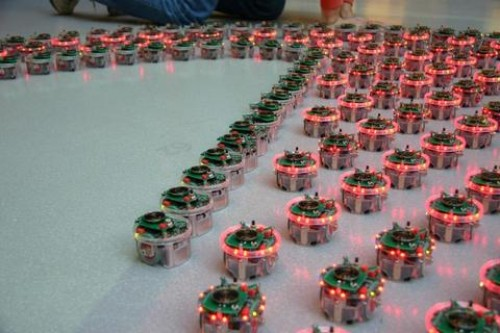
\includegraphics[scale=0.3]{e-puck_3.JPG}
        \end{column}
    \end{columns}
\end{frame}

\begin{frame}
    \frametitle{Krokové motory}
    \begin{columns}
        \begin{column}{0.5\textwidth}
            \begin{itemize}
                \item Dva krokové motory
                \item Tisíc kroků = jedna otáčka kola
                \item Jeden krok $\approx$ 0.13 mm
                \item Maximální rychlost jedna otáčka za sekundu
                \item Neklouzavá úprava
            \end{itemize}
        \end{column}

        \begin{column}{0.5\textwidth}
            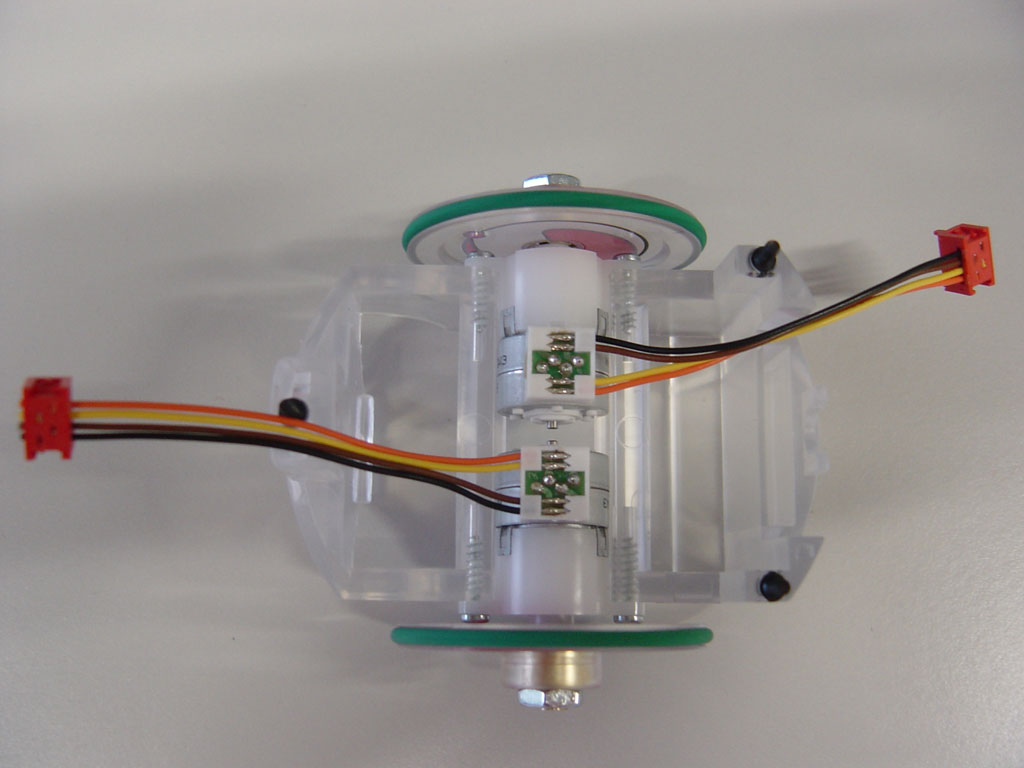
\includegraphics[scale=0.15]{mecanics.jpg}
        \end{column}
    \end{columns}
\end{frame}

\begin{frame}
    \frametitle{Speaker}
        \begin{itemize}
            \item Přehrává připravené zvuky (WAV)
            \item 5 zvuků zakompilovaných do firmware
        \end{itemize}
\end{frame}

\section{Připojení}

\begin{frame}
    \frametitle{Příprava PC}
    \begin{itemize}
        \item Potřeba funkční bluetooth
        \item Balíky {\tt bluez-firmware}, {\tt bluez-utils}
        \item Utilita na zaslání PIN ({\tt bluez-pin}, \ldots)
    \end{itemize}
\end{frame}

\begin{frame}[fragile]
    \frametitle{Nastavení rfcomm}
    \begin{block}{Získat adresu robota}
    \begin{minted}[firstline=2]{bash}
$
$ hcitool scan
Scanning ...
10:00:E8:52:C6:3E	e-puck_1055
    \end{minted}
    \end{block}

    \begin{block}{Nastavení {\tt /etc/bluetooth/rfcomm.conf}}
    \begin{minted}{yaml}
rfcomm2 {
    bind no;
    device 10:00:E8:52:C6:3E;
    channel 1;
    comment "e-puck_1055";
}
    \end{minted}
    \end{block}
\end{frame}

\begin{frame}[fragile]
    \frametitle{Vytvoření spojení}

    \begin{block}{Připojení pomocí {\tt rfcomm}}
    \begin{minted}[fontsize=\small]{text}
# rfcomm connect rfcomm2
Connected /dev/rfcomm2 to 10:00:E8:52:C6:3E on channel 1
Press CTRL-C for hangup
    \end{minted}
    \end{block}

    \begin{alertblock}{Možné chyby}
        {\em Can’t connect RFCOMM socket: Connection refused}
        \begin{itemize}
            \item Není spuštěná aplikace, která by předala PIN
        \end{itemize}
        {\em Can’t create RFCOMM TTY: Address already in use}
        \begin{itemize}
            \item Robot už je připojen
            \item Jiná aplikace s ním stále komunikuje
        \end{itemize}
    \end{alertblock}
\end{frame}

\begin{frame}[fragile]
    \frametitle{Nahrání firmware}
    \begin{itemize}
        \item Používá se {\tt epuckupload}
        \item Je potřeba mít aktivní připojení
        \item Robot dokáže přijímat nový firmware pouze pár sekund po restartu
    \end{itemize}
    \begin{block}{Postup při nahrávání}
        \begin{enumerate}
            \item Spuštění nahrávání
\begin{minted}[firstline=2]{bash}
            $
$ epuckupload -f BTcom.hex rfcomm2
\end{minted}

            \item Restartování robota
            \item Vyčkání na konec nahrávání
            \item Robot připraven k práci
        \end{enumerate}
    \end{block}

\end{frame}

\section{Komunikace}

\begin{frame}
    \frametitle{Komunikace}
    \begin{itemize}
    \item Kontrolní program běží v PC napsaný v Pythonu
    \item Příkazy jsou textové (binární) řetězce posílané přes sériové rozhraní
    \item V robotovi je upravený firmware BTcom, který pouze zpracovává příkazy
    \item Je potřeba aby bylo vytvořené připojení
    \end{itemize}
\end{frame}

\begin{frame}[fragile]
    \frametitle{Příklad ovládání}
    \begin{exampleblock}{Příklad zaslání příkazu}
    \begin{minted}[fontsize=\scriptsize]{python}
>>> from epuck import Controller
>>> controller = Controller("/dev/rfcomm2")
>>> controller.set_speed(100, 100)
>>> controller.get_speed()
(100, 100)
    \end{minted}
    \end{exampleblock}
    \begin{enumerate}
        \item Je vytvořen Controller, parametr je cesta k rozhraní kde
        je robot připojen
        \item Nastavena rychlost obou motorů na 100
        \item Zjištěna rychlost z robota
    \end{enumerate}

    Jde o synchronní komunikaci, program byl vždy zablokován dokud nedošla
    odpověď od robota.
\end{frame}

\begin{frame}[t]
    \frametitle{Druhy komunikace}
    \begin{columns}
        \begin{column}{.5\textwidth}
            \center{\large{Synchronní}}\vskip0.5cm
        \end{column}
        \begin{column}{.5\textwidth}
            \center{\large{Asynchronní}}
        \end{column}
    \end{columns}
    \vskip0.5cm

    \begin{columns}
        \begin{column}{.5\textwidth}
            \begin{itemize}
                \item Vždy víme, zda se příkaz provedl
                \item Transparentní komunikace
                \item Hned se dozvíme výsledek
                \item Pokud nastala chyba tak může zůstat v deadlocku
            \end{itemize}
        \end{column}
        \begin{column}{.5\textwidth}
            \begin{itemize}
                \item Není třeba čekat, než se příkaz vykoná
                \item Spolehlivá komunikace
                \item Zotavování z chyb
                \item Musíme si zvlášť říct o výsledek
            \end{itemize}
        \end{column}
    \end{columns}
\end{frame}

\begin{frame}[fragile]
    \frametitle{Asynchronní komunikace}
    \framesubtitle{Příklad programu}
    \begin{exampleblock}{Ukázka kódu}
    \begin{minted}[fontsize=\scriptsize]{python}
from epuck import Controller

controller = Controller("/dev/rfcomm2", asynchronous=True)
photo_request = controller.get_photo()
while not photo_request.response_received():
    foo()
photo = photo_request.get_response()
    \end{minted}
    \end{exampleblock}

    \begin{itemize}
        \item Místo odpovědi získáme jen handler
        \item Je možné zkontrolovat zda-li už přišla odpověď
        \item Než přijde odpověď, tak je možné dělat cokoli jiného
    \end{itemize}
\end{frame}

\begin{frame}[fragile]
    \frametitle{Asynchronní komunikace}
    \framesubtitle{Callback}
    \begin{itemize}
        \item Pro zpracování odpovědi je možné mít speciální funkci
        \item Každý příkaz má parametr callback, což je funkce
        \item Callback je zavolán hned po přijetí odpovědi
        \item Callback může být použit pro modifikaci odpovědi:
        \mint[fontsize=\scriptsize]{python}|vysledek_get_response = callback(odpoved_od_robota)|
    \end{itemize}
    \begin{exampleblock}{Ukázka callback metody}
    \begin{minted}[fontsize=\scriptsize]{python}
from epuck import Controller

controller = Controller("/dev/rfcomm2", asynchronous=True)
controller.get_photo(callback=lambda img: img.show())
    \end{minted}
    \end{exampleblock}

\end{frame}

\section{Přehled příkazů}

\begin{frame}
    \frametitle{Příkazy}
    \begin{itemize}
        \item Třída {\tt Controller} obsahuje  příkazy pro ovládání všech
        sensorů a akčních členů robota
        \item Každá akce je pouze zavolání jedné metody
        \item Při synchronní komunikaci vrací metody rovnou výsledek
        \item Při asynchronní komunikaci vrací handler.
        \item Bližší informace v dokumentaci
    \end{itemize}
\end{frame}

\begin{frame}
    \frametitle{Příkazy}
    \framesubtitle{Přehled}
    \begin{itemize}
        \item Motory
        \begin{itemize}
            \item \mint{python}|set_speed(left, right)|
            \item \mint{python}|get_speed()|
            \item \mint{python}|set_motor_pos(left, right)|
            \item \mint{python}|get_motor_pos()|
        \end{itemize}
        \item IR senzory
        \begin{itemize}
            \item \mint{python}|get_proximity_sensors()|
            \item \mint{python}|get_ambient_sensors()|
            \item \mint{python}|calibrate_sensors()|
        \end{itemize}
        \item LED
        \begin{itemize}
            \item \mint{python}|set_body_led(on)|
            \item \mint{python}|set_front_led(on)|
            \item \mint{python}|set_leds(on)|
            \item \mint{python}|set_led(led_no, on)|
        \end{itemize}
    \end{itemize}
\end{frame}

\begin{frame}
    \frametitle{Příkazy}
    \framesubtitle{Přehled}
    \begin{itemize}
        \item Kamera
        \begin{itemize}
            \item \mint{python}|set_camera(mode, width, height, zoom)|
            \item \mint{python}|get_camera()|
            \item \mint{python}|get_photo()|
        \end{itemize}
        \item Přepínač na robotovi
        \begin{itemize}
            \item \mint{python}|get_turning_switch()|
        \end{itemize}
        \item Akcelerometr
        \begin{itemize}
            \item \mint{python}|get_accelerometer()|
            \item \mint{python}|get_raw_accelerometer()|
        \end{itemize}
        \item Zvuk
        \begin{itemize}
            \item \mint{python}|play_sound(sound_no)|
            \item \mint{python}|get_volume()|
        \end{itemize}
        \item Restart nebo zastavení
        \begin{itemize}
            \item \mint{python}|reset()|
            \item \mint{python}|stop()|
        \end{itemize}
    \end{itemize}
\end{frame}
\section{Ukázky programů}

\begin{frame}[fragile]
    \frametitle{Následování světla}
    \begin{itemize}
        \item Využity IR senzory
        \item Robot se pohybuje za světlem
        \item Je potřeba zdroj IR světla (svíčka, \ldots)
    \end{itemize}
    \begin{exampleblock}{Zdrojový kód 1/3}
    \begin{minted}[fontsize=\scriptsize,linenos=true]{python}
import logging
import time
import sys
import signal

from epuck.controller import Controller

logging.basicConfig(level=logging.WARNING)

c = Controller("/dev/rfcomm2", asynchronous=True)
    \end{minted}
    \end{exampleblock}
\end{frame}

\begin{frame}[fragile,t]
    \frametitle{Následování světla}
    \begin{exampleblock}{Zdrojový kód 2/3}
    \begin{minted}[fontsize=\scriptsize,linenos=true]{python}
# Signal handler to cleanup after shutdown
def handle_signal(signum, frame):
    r = c.stop()
    r.join()
    sys.exit(0)

# SIGINT is interrupt signal sent by CTRL+C
signal.signal(signal.SIGINT, handle_signal)

while True:
    # Read ambient light sensors
    r = c.get_ambient_sensors().get_response()

    front_side = r["L10"] + r["R10"]
    left_side = r["L45"] + r["L90"]
    right_side = r["R45"] + r["R90"]
    \end{minted}
    \end{exampleblock}
\end{frame}

\begin{frame}[fragile,t]
    \frametitle{Následování světla}
    \begin{exampleblock}{Zdrojový kód 3/3}
    \begin{minted}[fontsize=\scriptsize,linenos=true]{python}
    # The light source is straight ahead
    if front_side < left_side and front_side < right_side:
        c.set_speed(500, 500)
    elif left_side < right_side:
        c.set_speed(-500, 500)
    else:
        c.set_speed(500, -500)

    time.sleep(0.1)

    \end{minted}
    \end{exampleblock}
\end{frame}

\begin{frame}
    \frametitle{LED}
    \begin{itemize}
        \item Pouze efekty s LED
        \item Přepínač na robotovi využit pro různé režimy
    \end{itemize}
\end{frame}

\begin{frame}
    \frametitle{Vyhýbání se překážkám}
    \begin{itemize}
        \item Jednoduchý program na principu Braitenberg vehicle
        \item Výstup na akčních členech je ovlivněn pouze hodnotou senzorů
    \end{itemize}
\end{frame}

\begin{frame}
    \frametitle{Detekce obličejů}
    \begin{columns}
        \begin{column}{0.6\textwidth}
            \begin{itemize}
                \item Použita kamera a OpenCV knihovna
                \item Program každých pár sekund sejme obrázek a snaží se na něm nalézt obličej
            \end{itemize}
        \end{column}

        \begin{column}{0.4\textwidth}
            
\includegraphics[scale=1]{face1.jpg}
            \hskip1cm
            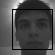
\includegraphics[scale=1]{face2.jpg}
        \end{column}
    \end{columns}
\end{frame}

\begin{frame}
    \frametitle{Evoluce}
    \begin{itemize}
        \item Experiment s knihovnou PyEvolve
    \end{itemize}
\end{frame}

\section{Závěr}
\begin{frame}
    \frametitle{Odkazy}
    \begin{block}{Stránky e-puck}
    \small
    \url{http://www.e-puck.org}
    \end{block}
    \begin{block}{Bootloader}
    \small
    \url{http://svn.gna.org/viewcvs/e-puck/trunk/tool/bootloader/computer_side/multi_platform/}
    \end{block}
    \begin{block}{Dokumentace}
    \small
    \url{http://e-puck.davidmarek.cz}
    \end{block}
    \begin{block}{Projekt}
    \small
    \url{http://github.com/davidmarek/E-Puck-Algorithms-Library}
    \end{block}
\end{frame}


\end{document}
